\chapter{発話内容を考慮した偽音声検出}\label{ch:spc_cnt}
\section{目的}\label{sec:cnt_pur}
\subsection{形式の位置づけ}
音声を入力とする話者認識(Speaker Recognition)には、話者識別(Speaker Identification)と話者照合(Speaker Verification)という2種類の形式がある \cite{FURUI1997859,628714,5745552}。
\cref{fig:speaker_recog}は2種類の形式の違いを示す。

\begin{figure}[p]
    \centering
    \begin{minipage}{0.9\linewidth}
        \centering
        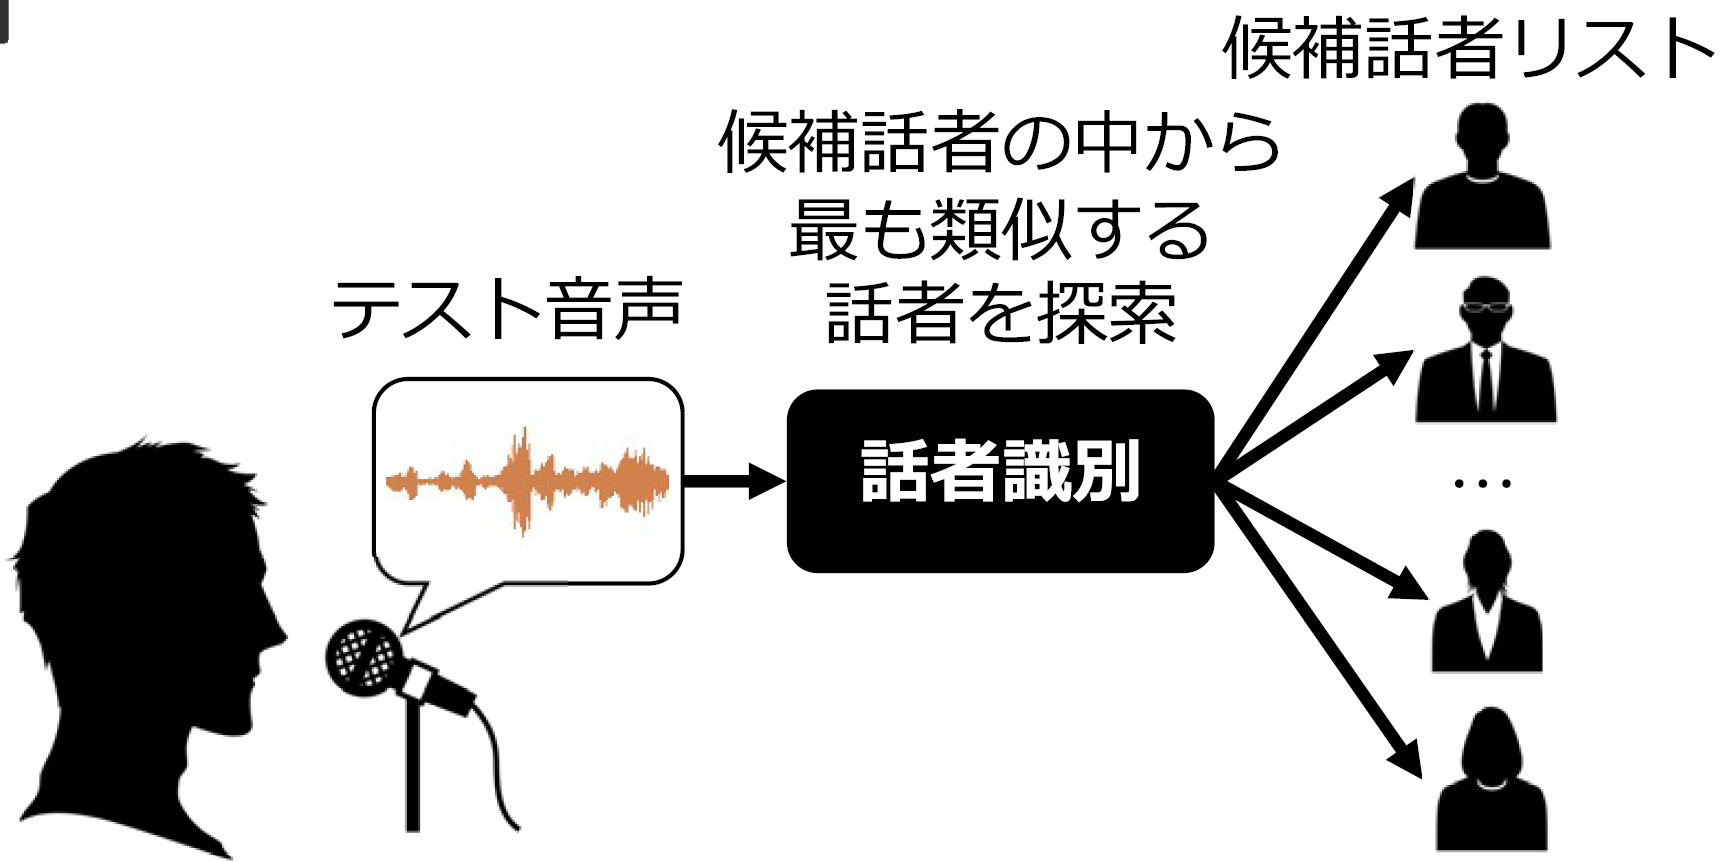
\includegraphics[width=0.8\linewidth]{figures/sd.png}
        \subcaption{話者識別}
    \end{minipage}
    \begin{minipage}{0.9\linewidth}
        \centering
        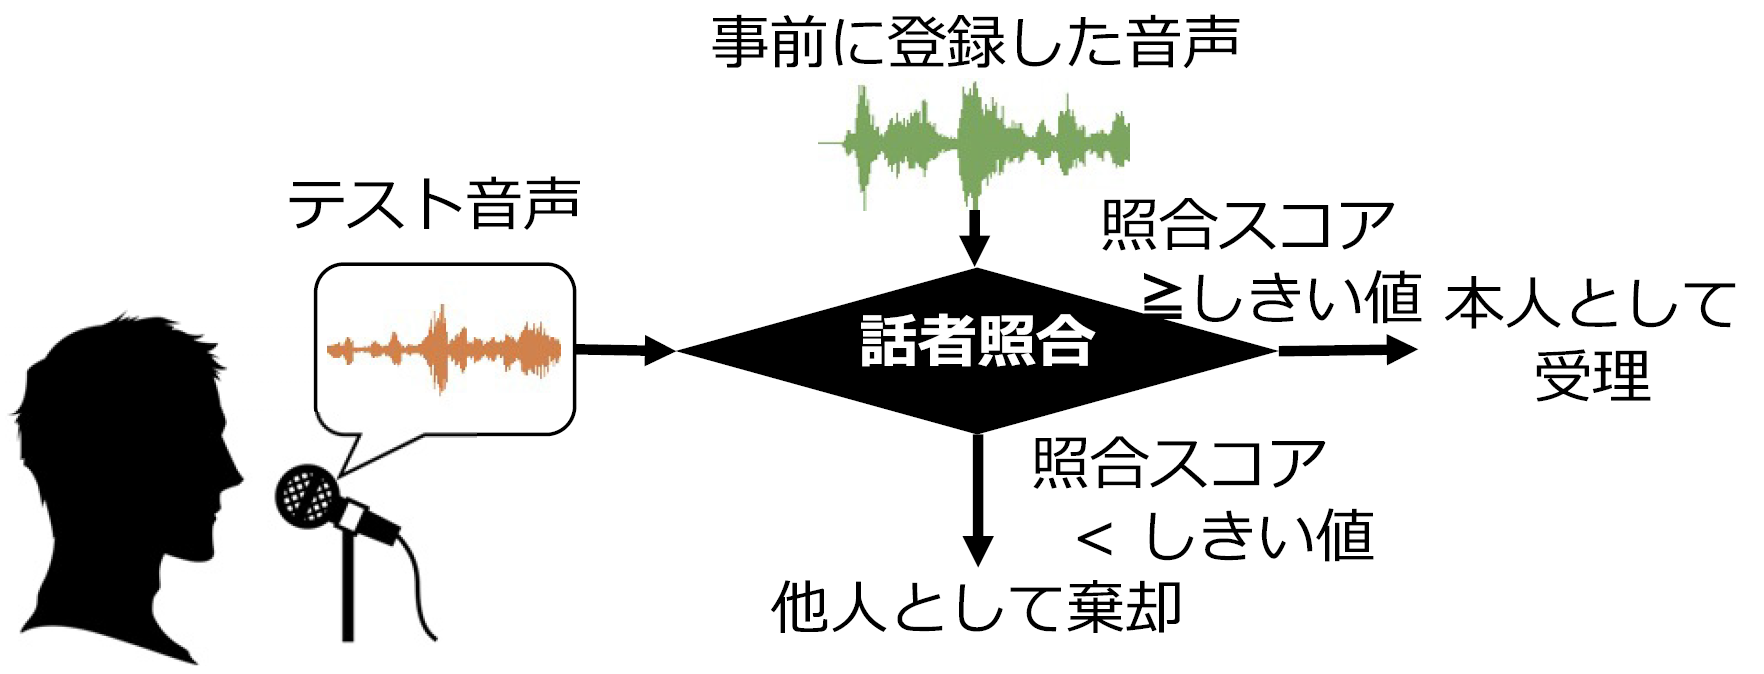
\includegraphics[width=0.8\linewidth]{figures/sv.png}
        \subcaption{話者照合}
    \end{minipage}
    \caption{話者認識の形式 \cite{俵直弘2022}}
    \label{fig:speaker_recog}
\end{figure}

話者識別は事前に登録した複数の候補者の中から提示された音声の話者を探索する1対nの推定問題であるのに対し、
話者照合では,提示された二つの音声が同一話者によるものか否かを推定する1対1の照合問題として定義する \cite{俵直弘2022}。
識別では、未知の話者を既知の話者のデータベースと比較し、最もよく一致する話者を識別結果として与える。
一方で照合では、音声サンプルが主張された人物によって話されたかどうかを判断するタスクと言える \cite{1561284}。
よって、本研究で行うなりすまし偽音声の検出は、話者照合に該当する。

また,話者認識は,登録時と照合時で同じ内容の音声を用いるテキスト依存型(text-dependent)と,
登録時と照合時で異なる内容の音声を用いるテキスト独立型(text-independent)に分類される \cite{俵直弘2022}。
ASVspoofにおけるなりすまし検出では、テキスト依存型の形式を取っている。
読み上げる音声は本人・偽いずれも新聞記事から引用した同一の文章を読み上げているため、
実際にSNS上で偽音声による偽情報が投稿された状況から乖離がある。
よって本研究では、テキスト独立型の話者照合を行う。

\subsection{検出対象の位置付け}
本研究の目的は、偽情報を話すなりすまし音声(偽音声)を自動で検出することである。
偽情報を話す偽音声には内容の確からしさと音声そのものの本人性という2種類の概念をもつ。
話す内容の確からしさは、事実か・偽情報かの2種がある。
本来ではこの2種類以外に事実ではないものの意図的に発信されたものではない誤情報もあるが、本章では考慮しない。
本人性は本人が話すか・本人以外がなりすましているかの2種がある。
本人以外がなりすます場合では機械による合成処理を含まない場合(声真似等)もあるが、
意図的に社会に不安を与える行為として行われにくいと考えられるため本章では考慮しない。

よって、偽情報を話すなりすまし音声を検出する場合、モデルへ入力する対象は内容の確からしさと本人性から以下の4種類が挙げられる。

\begin{itemize}
    \item 偽情報を話すなりすまし音声(検出したい対象)
    \item 事実を話すなりすまし音声
    \item 偽情報を話す本人音声
    \item 事実を話す本人音声
\end{itemize}

また、\cref{fig:twoPerspective}は内容信憑性・本人性の2種類による配置を表す。

\begin{figure}[p]
    \centering
    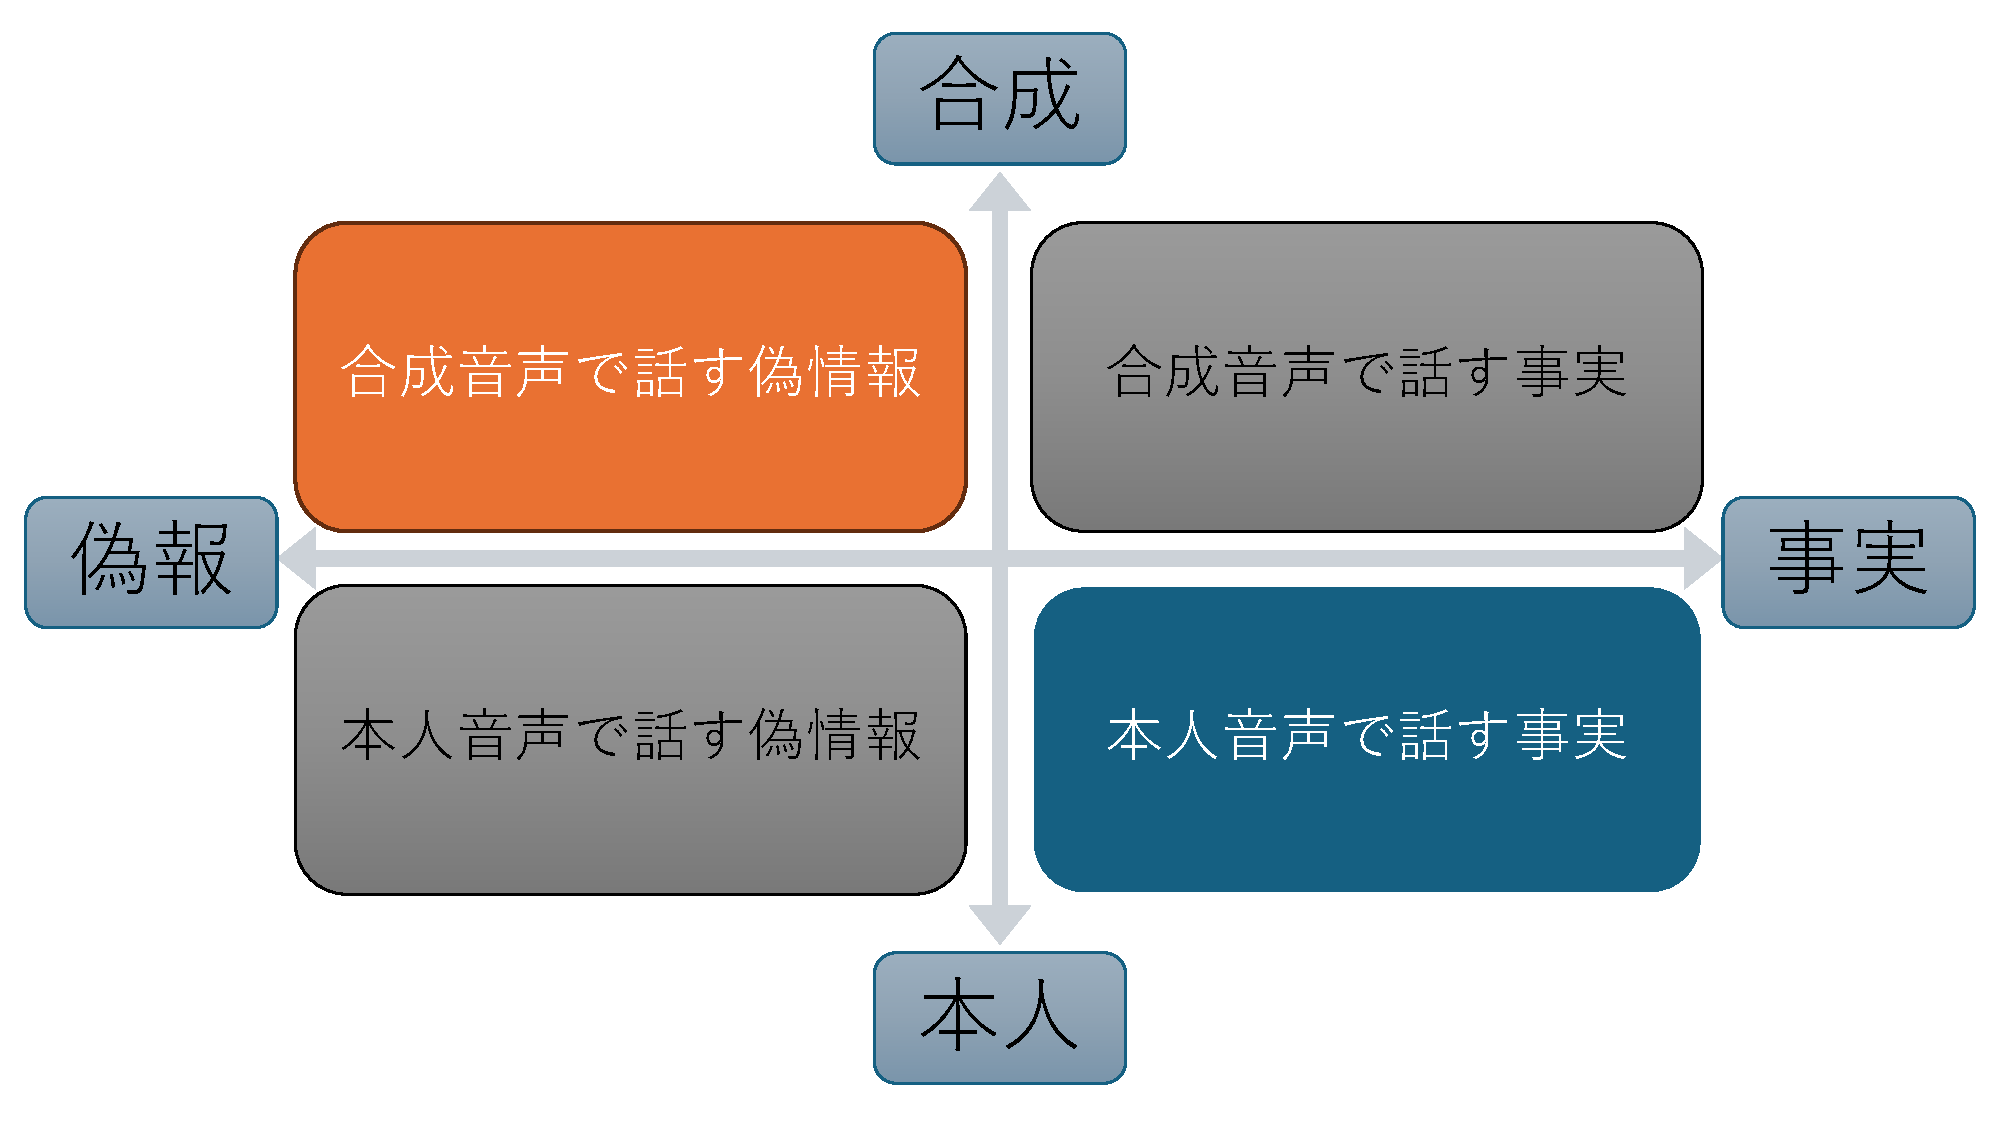
\includegraphics[width=\linewidth]{figures/D論概念図.pdf}
    \caption{発話内容の信憑性と、発話者の本人性による音声の種類。本研究では合成音声で話す偽情報と本人音声で話す事実の2種類に着目する。}
    \label{fig:twoPerspective}
\end{figure}

事実を話す本人音声は、検出したい対象である偽情報を話すなりすまし音声とは内容の確からしさ及び本人性の両方において、対極に位置する概念である。
本研究では、実験にて検出すべきでない対象として扱う。

事実を話すなりすまし音声は、主にマスメディアによるニュース記事の読み上げ(AIアナウンサー)が例として挙げられる\cite{nhk2020,nhkAnnual2020}。
マスメディアによる運用が行われているため、SNS上に投稿された場合は性質上一定の信憑性が見込まれて検出の必要性が薄いと判断し、本研究では扱わないこととした。

偽情報を話す本人音声は実際の例として演説や講演会、そして特殊詐欺などが挙げられる。
この場合は実際に話さなければならない都合上、SNS上での事例が偽情報を話すなりすまし音声に比べて変化が少ないほか、
先行研究として特殊詐欺の自動検出を目指した事例 \cite{近野恵2023}があるため、
検出したい対象に対して重要度が比較的高くないと判断し、本研究では扱わないこととした。

以上から、本研究の目的は事実を話す本人音声と偽情報を話すなりすまし音声の2種類の音声から検出を行う。

\section{手法}\label{sec:cnt_mtd}
本節では、虚偽の主張を発信する偽音声を自動検出するための提案手法を紹介する。
我々の手法には、波形を分析する部分と、発話内容を評価する部分の2つの異なる処理部分が組み込まれている。
\cref{fig:structure}は、我々の提案する手法の構造を示している。これより各部の詳細を説明する。

\begin{figure}[p]
    \centering
    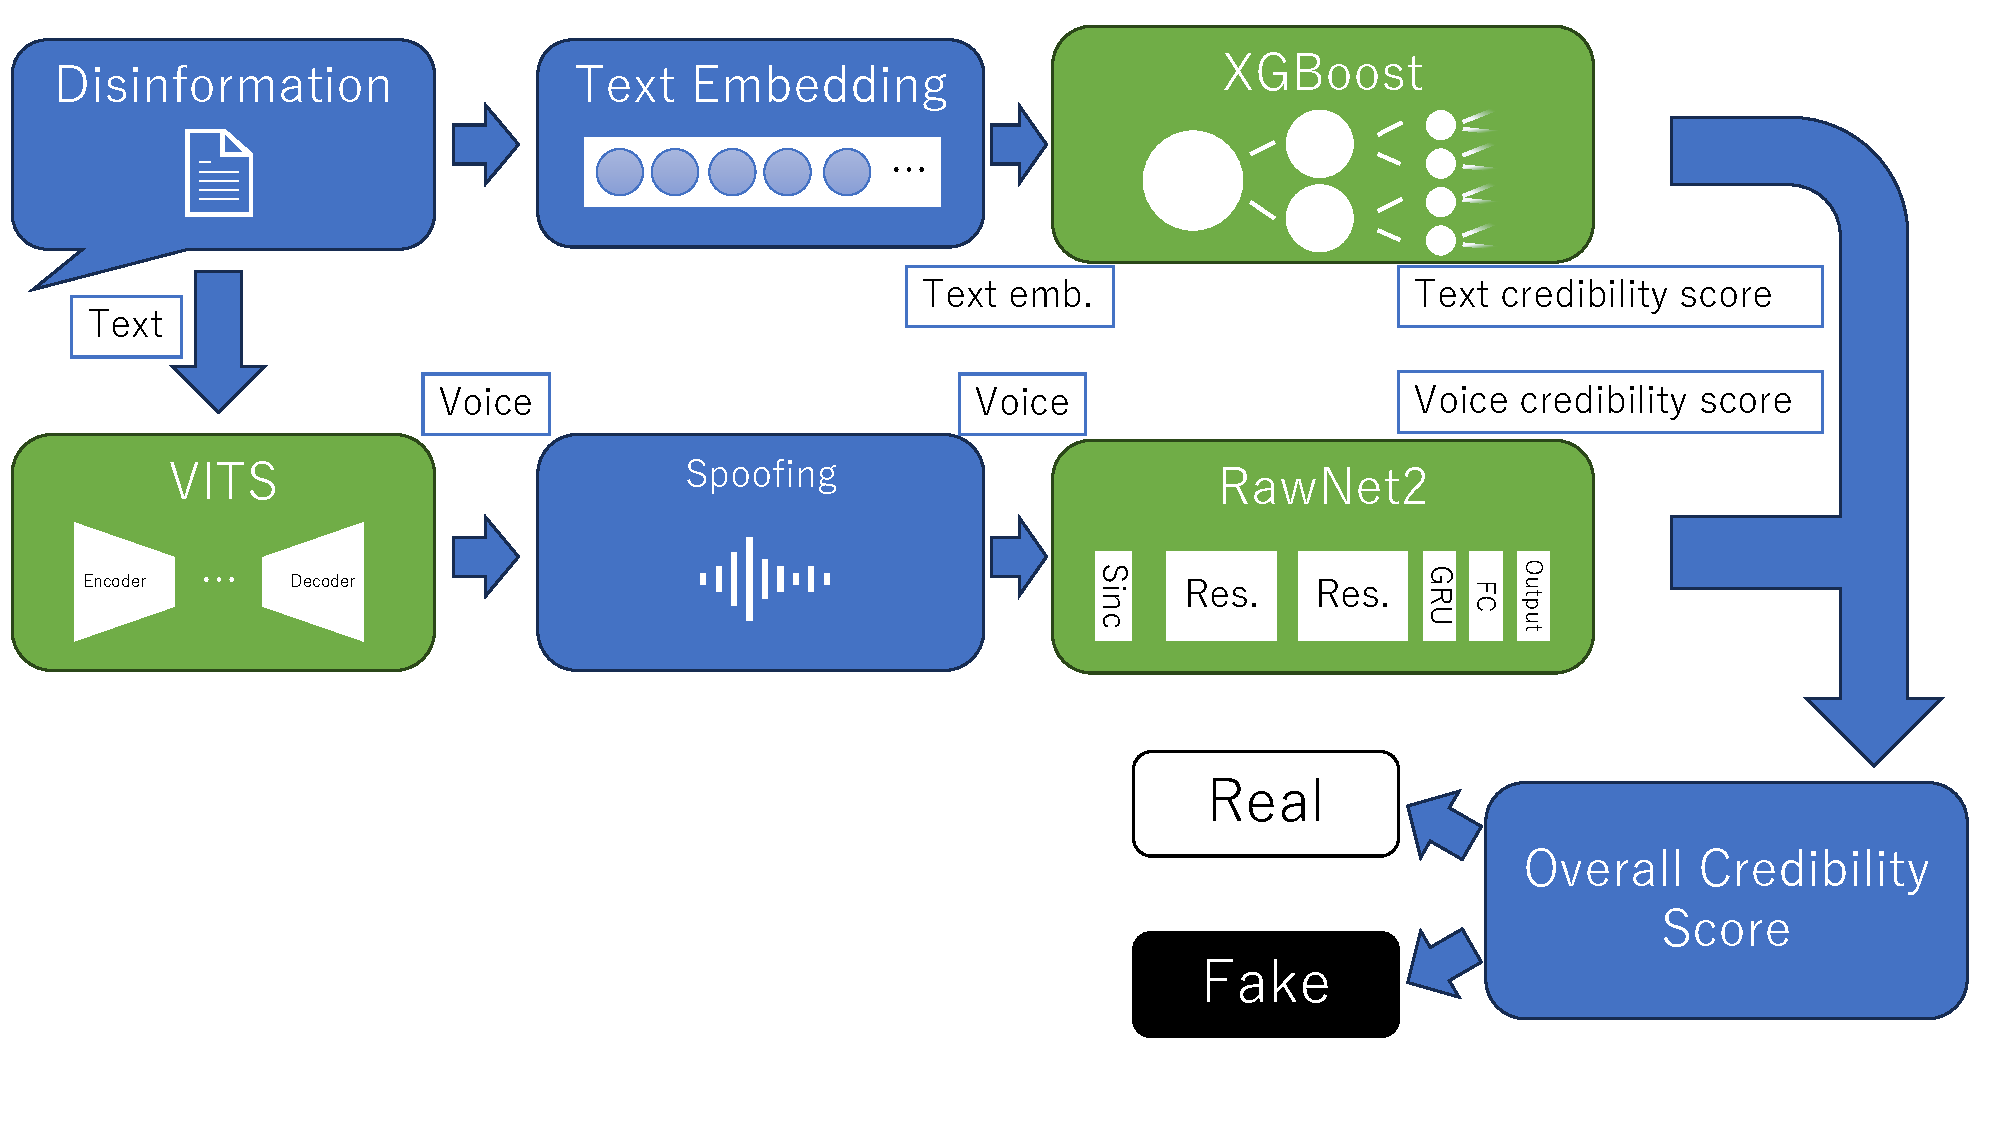
\includegraphics[width=\linewidth]{figures/Structure.pdf}
    \caption{データセットの生成から提案手法が行う分析の流れ。}
    \label{fig:structure}
\end{figure}

\subsection{波形分析}
偽音声の波形を直接分析する形式として、RawNet2とRawBoost、そして本実験ではSSL-Antispoofingを採用した。

\subsubsection{RawNet2}
音声波形を直接扱う既存手法として、
ASVspoofにてベースラインとして提供された \cite{WANG2020101114}RawNet2を採用した。
RawNet2はもともとRawNet \cite{jung19b_interspeech}から拡張された手法で、
いずれも発話レベルの特徴抽出と特徴拡張を単一モデルで完結させた上で分類を行う。
今回採用したRawNet2の構造は\cref{tb:rawnet2}の通りである。

RawNet2はRawNetモデル \cite{jung19b_interspeech}の拡張版である。
どちらのモデルも直接波形を分析して合成音声の疑いの強さを出力とするEnd-to-endの分類器として動作する \cite{jung19b_interspeech}。
RawNet2のフレームワークの最初のレイヤーは、SincNet \cite{8639585,ravanelli19_interspeech}として導入されたSinc-convolutionレイヤーを利用している。
SincNetは畳み込みニューラルネットワーク(CNN)を採用し、sinc関数に似たバンドパスフィルターを用いて入力波形をフィルターする。
第2層は残差ブロックからなり、バッチ正規化(BN)、LeakyReLU \cite{maas2013rectifier}、畳み込み層、最大値プーリング、特徴マップスケーリング(Feature Map Scaling, FMS)を含む。
FMSは[39]で提案され、シグモイド活性化 \cite{jung20c_interspeech}を持つ注意層と同様の機能を持つ。
出力層は二値分類用に設計されており、合成によるなりすました音声と本人の音声を区別する。
このモデルは、GitHub リポジトリにある ASVspoof のベースライン設定に従って、重み付けされたカテゴリ横断エントロピーを損失関数として利用する。
これは本物の声と偽物の声を区別するための二値分類タスクであることから、本モデルの損失 $ L_{RN} $は以下の式で決定される。

\begin{equation}
    L_{RN}(y, \hat{y}) = -0.1 * y \log{\hat{y}} - 0.9 * (1-y) \log{(1-\hat{y})}
\end{equation}

この式では、$y$はラベルの値であり、$y=0$は本人に、$y=1$はなりすまし偽音声に該当する。
$\hat{y}$はRawNet2による出力に該当し、log関数にかけられている。
定数0.1及び0.9はASVspoof内での学習におけるラベル分布を根拠とする重み付けとして設定されている \cite{yamagishi21_asvspoof}。

%\begin{figure}[ht]
%    \centering
%    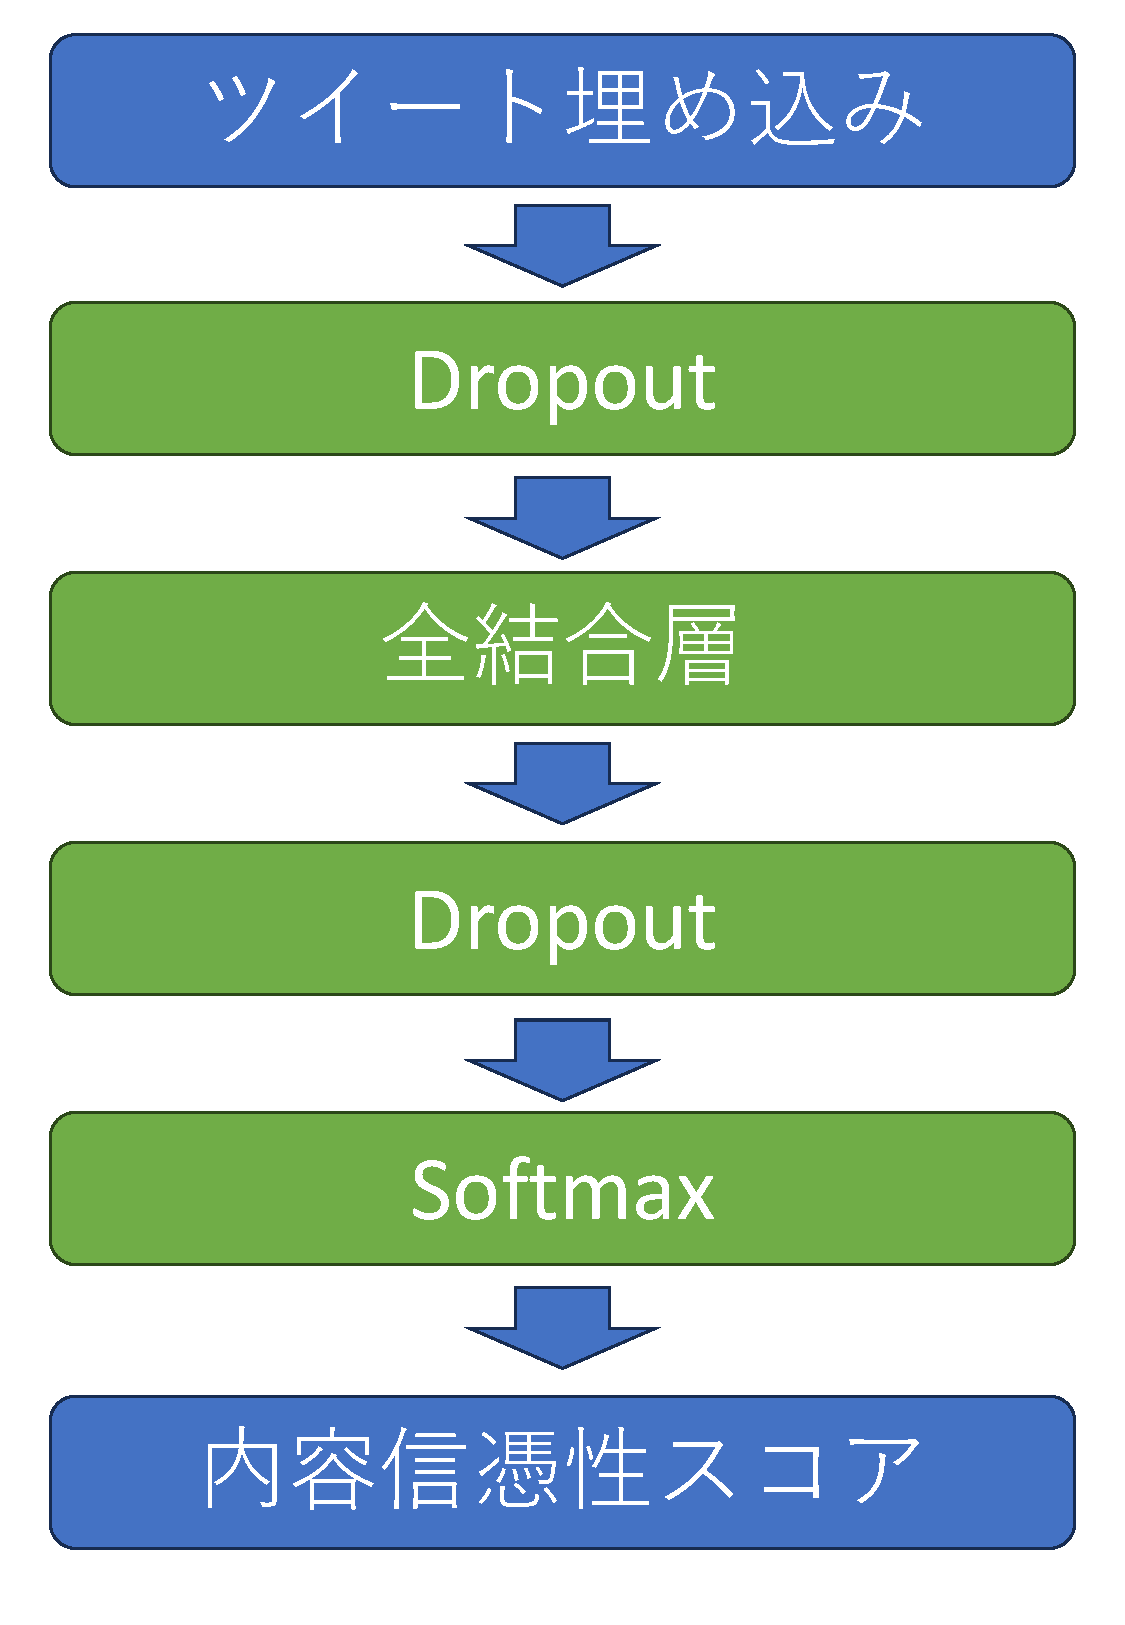
\includegraphics[width=0.5\textwidth]{./figures/ieice_nnfig.pdf} %TODO 次元情報追加
%    \caption{提案手法における内容信憑性評価部分。}
%    \label{fig:content}
%\end{figure}

\begin{table}[p]
    \centering
    \caption{ASVspoof 2019以降で採用されている \cite{9414234,yamagishi21_asvspoof}RawNet2の構造}
    \begin{tabular}{l@{}c@{}l}\hline
        層 & 入力 & 出力形式 \\\hline\hline
        \multirow{3}{*}{調整済Sincフィルタ} & 畳み込み(129,1,128) & \multirow{3}{*}{(21290, 128)}\\
        & 最大値プーリング(3) &\\
        & バッチ正規化(BN) \& LeakyReLU &\\\hline
        \multirow{6}{*}{残差ブロック}&\multirow{6}{*}{$\left\{\begin{array}{c}\rm{BN \& LeakyReLU}\\
        \rm{畳み込み(3,1,128)}\\
        \rm{BN \& LeakyReLU}\\
        \rm{畳み込み(3,1,128)}\\
        \rm{最大値プーリング(3)}\\
        \rm{特徴マップスケーリング(FMS)}\\\end{array}\right\}$}& \multirow{6}{*}{(2365, 128)}\\ \\ \\ \\ \\ \\\hline
        \multirow{6}{*}{残差ブロック}&\multirow{6}{*}{$\left\{\begin{array}{c}\rm{BN \& LeakyReLU}\\
        \rm{畳み込み(3,1,128)}\\
        \rm{BN \& LeakyReLU}\\
        \rm{畳み込み(3,1,128)}\\
        \rm{最大値プーリング(3)}\\
        \rm{FMS}\\\end{array}\right\}$}& \multirow{6}{*}{(29, 512)}\\ \\ \\ \\ \\ \\\hline
        ゲート付き回帰型ユニット&GRU(1024)&(1024)\\\hline
        全結合層&1024&(1024)\\\hline
        Output&1024&2\\\hline
        %& Maxpooling(3) &\\
    \end{tabular}
    \label{tb:rawnet2}
\end{table}

\subsubsection{RawBoost}
さらに、RawNet2とは別の手法としてRawBoost \cite{9746213}を採用した。
RawBoostは、学習にて音声内のノイズ対策として独自のデータ拡張手法を取り入れている \cite{9746213}。
このモデルを使用したのは、ASVspoofにおけるRawNet2を含むベースラインよりも良好なスコアが \cite{9746213}にて報告されたためである。
具体的なデータ拡張として、
(1)線形および非線形の畳み込みノイズ(符号化、圧縮、および送信プロセス中に導入されるノイズを再現している)、
(2)クリッピングやデバイス(マイクやアンプなど)の非最適動作などのインパルス信号依存の付加ノイズ、
(3)単一の有限インパルス応答フィルタを適用することによる定常信号非依存のノイズ付加が導入されている \cite{9746213}。
さらに、学習時の損失関数として、GitHubリポジトリ \footnote{\url{https://github.com/TakHemlata/RawBoost-antispoofing}}で提供されている仕様に従って、同じ重み付きクロスエントロピー損失を採用した。

\subsubsection{SSL Anti-spoofing}
本実験では、SSL Anti-spoofingも導入した。
RawBoostと同じくTakら \cite{tak2022automatic}によって提案された手法である。
RawNet2との違いとして入力を直接受ける部分としてSincフィルタではなくwav2vec 2.0 \cite{NEURIPS2020_92d1e1eb}を導入し、自己教師あり学習を取り入れている。

この手法はASVspoof2021の開催後に行われたLogical Access及びDeep Fakeにおける事後タスクにて全体で最も優秀な成績を収めている \cite{10155166}。

\subsection{埋め込みによる発話内容の分析}
音声の内容を考慮するために、MuMiNデータセット \cite{10.1145/3477495.3531744,NielsenMcConville2022}から得られるツイート埋め込みを活用する。
データセット内でテキスト特徴としてすぐに使えるので、本研究で使用した。
この埋め込みはBART-large-CNN \cite{lewis-etal-2020-bart}を使って生成される。
ツイート埋め込み用の分類器としてXGBoost \cite{10.1145/2939672.2939785}を採用した。
今後のの計画には、ディープニューラルネットワークモデルを組み込むことが含まれている。
また、自動音声認識モデルを統合し、ソーシャ ルメディアのコンテキスト内で DeepFakeの声を検出する包括的なアプローチを取り入れることも視野に入れている。
損失$L_{emb}$は、Chen Tら \cite{10.1145/2939672.2939785}で詳しく説明されているように、重み付き二乗損失の平均として計算され、以下のように定義される。

\begin{align} 
        L_{emb} = \sum_l (\hat{y_i}, y_i) + \sum_k \Omega (f_k) \\
        \text{where}~\Omega (f) = \gamma T + \frac{1}{2} \lambda ||w||^2
\end{align}

この式では、$y_i$は$i$番目のラベルの値を示し、$\Omega$は葉ノードの数($T$)と重みのL2ノルムからなり、正則化項として総和がモデルの複雑さにペナルティを与える \cite{10.1145/2939672.2939785}。
定数$\gamma$および$\lambda$は今回では公式ドキュメント \footnote{\url{https://xgboost.readthedocs.io/en/stable/parameter.html}}にてモデルのデフォルト値とされていた0として実装した。
つまり今回では発話内容学習による損失は、事実上重みづけ二乗平均として算出される。
パラメータチューニングによる最適化は今後の手法改善における余地となっている。

\subsection{波形と内容検証結果の統合}
最終的な音声信憑性スコア$c_f$は波形および内容における検証結果スコアの平均によって導かれる。

\begin{equation}
    c_f = \alpha c_w + (1 - \alpha) c_{emb}
\end{equation}

$\alpha$は$[0, 1]$の範囲であり、波形分析による信憑性 $c_w$とテキスト埋め込みの分析による信憑性$c_{emb}$に対する係数として作用する。
$c_w$は波形分析を行うRawNet2の最終的な出力から $[0,1]$の範囲で正規化がなされている。

後述の波形分析単体で行う実験では $\alpha = 1$として扱ったほか、
実際に内容も考慮して検出を行う実験では $\alpha = 0.5$とした。
この判断は、SNSにおける偽情報を話すなりすまし偽音声を検出するための新しいアプローチを提示するという、我々の主要な目的と一致する。
確かにRawNet2の平均スコアとディープニューラルネットワークを介したテキスト埋め込みを統合する代替アプローチも考えられるが、この方法はかなりの計算資源と時間を必要とする。
即時性が求められるSNS環境における現実的なシナリオを考慮し、我々は効率性を重視するため、加重二乗損失の平均値のみに基づいて損失を計算する。

\section{予備実験: 既存手法における新型音声合成手法への対応}
\subsection{データセット作成手法}\label{ssc:spc_ds}
発話内容を考慮したモデルに分類させるため、
事実に基づく情報を読み上げる音声と事実と異なる偽情報を読み上げる音声を用意した。
読み上げる対象はMuMiNデータセットが保有する英語の偽情報ツイートとした \cite{10.1145/3477495.3531744}。
選定理由はデータセットからツイート文章とともに内容を埋め込みに変換した情報も得られることから、後述の提案手法への接続が容易に実現できるためである。

読み上げ手法はVITSを採用した \cite{pmlr-v139-kim21f}。
\cref{ch:rel_res}で紹介した文章から音声を生成するText-To-Speechの形式であることと、
生成性能が良好である点が示されている点、
そして音声生成学習においてLJSpeechデータセット \cite{ljspeech17}による事前学習済みモデルが公開されており、生成への活用が容易である点から採用した。

なお実験で使用するにあたって、SNS上での投稿を想定して音声が3分以内に収まるように
英単語数の上限を480に設定し、超過分は切除した上でVITSによる音声生成を行った。
ただしTwitterツイートは仕様上480文字までの制限があるため、今回実験で使用した音声長は最長でも24秒である。
データセットの統計は\cref{tb:dataset}の通りである。

\begin{table}[h]
    \centering
    \caption{実験で使用した偽音声データセットの統計}
    \begin{tabular}{lc}\hline
        項目 & 値\\\hline\hline
        ツイート件数 & 722\\
        最大単語数 & 50\\
        平均単語数 & 24.9\\
        平均音声長 [\si{s}] & 8.2\\\hline
    \end{tabular}
    \label{tb:dataset}
\end{table}

\subsection{検出手法}
発話内容を考慮したモデルを構築するために、文章埋め込みを入力にもつモデルを音声波形を扱う既存手法に追加する手法を提案する。提案手法全体の概観は\cref{fig:allmodel}の通りである。

提案手法は、MuMiNデータセット内にてツイートに書かれた言語に対応したBERTベースの変換モデル \cite{lewis-etal-2020-bart}を適用したツイート埋め込みを入力に、ニューラルネットワークを介して内容の信憑性を評価する。
具体的な内容信憑性評価部分の流れは\cref{fig:content}の通りである。
最終的な信憑性スコアは音声信憑性評価による出力と内容信憑性評価による出力の平均値とした。
追加部分が音声を入力に使わなかった理由として、TTSによって得た合成音声は自動音声認識(Automatic Speech Recognition; ASR)による書き起こしが容易に得られることが想定でき、省略可能と考えたためである。
%今後VCによる変換も対象に入れる場合も想定し、音声を入力としてASRから発話内容を得る形への拡張も想定している。

\section{予備実験: 新型音声合成手法に対する既存検出手法の検証}
\subsection{実験内容}
\subsection{結果}
\section{本実験: 発話内容考慮による検出性能改善の検証}\label{sec:cnt_main}
\subsection{実験内容}
発話内容も含めて音声の信憑性を評価する手法の有効性を検証するために、
同じ合成音声でありながら事実に基づく情報とそうでない情報を真偽分類する実験を行った。
具体的なデータセット取得の手続き\cref{ssc:spc_ds}を参照のこと。
なおデータセット内の各ツイートのラベルはfactual/fakeの2種類である。
RawNet2は事前学習としてASVspoof 2021にて提供されたオンライン環境を想定した音声セットであるDFデータセットで学習済のものを使用した。
これはオンライン上に投稿された状況を想定した2019年までに提案された手法による合成音声から構成される。
また内容信憑性評価部分も含めた学習からテストまでの流れは学習/検証/テストの比率0.7:0.1:0.2の割合で分割して行った。学習エポック数は10だった。

評価指標は等価エラー率(Equal Error Rate; EER)を採用した。
これは真偽判断の閾値を本人拒否率(False Rejection Rate; FRR)と他人受入率(False Acceptance Rate; FAR)が同値になるように調整したときのエラー率を示したものである。
この2値は以下の式によって導出される。
\begin{eqnarray}
    FRR = \frac{FN}{FN+TP} \\
    FAR = \frac{FP}{FP+TN}
\end{eqnarray}

今回の実験でTP(True Positive)は偽情報を話す合成音声を正しく虚偽と検出できた回数を示し、
FN(False Negative)は偽情報を話す合成音声を誤って事実と分類した回数を示し、
FP(False Positive)は事実を話す合成音声に誤って虚偽と検出した回数を示す。

実験では提案手法の有効性を確認するために、
音声のみで分類を行った場合の結果と比較した。

\subsection{結果}\label{sec:cnt_res}
実験によって音声を分類した結果は\cref{tb:result}の通りである。
音声のみを入力として扱った場合、等価エラー率(EER)は50.7\%だった。
EERが50\%であることは、コイントスによって決定することとと同義であることから、
%2019年までの音声合成手法によって訓練されたRawNet2では、
%VITSによる音声を識別することが限りなく難しいことを示している。
%自明であるが、
内容の真偽に関係なく、発話音声か合成音声かを区別するように訓練されたRawNet2では、
内容が真の合成音声と内容が偽の合成音声とを区別することはできなかった。
一方で、内容評価を行う部分を付加した場合、
EERは44.59\%まで改善がみられた。

\begin{table}[h]
    \caption{事実に基づく情報と事実と異なる偽情報を話す合成音声を真偽分類した結果。}
    \centering
    \begin{tabular}{l|c}\hline
       モデル形態 & 等価エラー率(EER)[\%] \\\hline\hline
       音声評価 (RawNet2)のみ & 50.7\\
       提案手法(内容評価を伴う場合) & \textbf{44.6}\\\hline
    \end{tabular}
    \label{tb:result}
\end{table}

\section{考察}\label{sec:cnt_evl}

